\section{Aquisição de Imagem}

\begin{frame}[allowframebreaks]
  \frametitle{CCD Chip}
  \begin{figure}[h!]
  \centering
  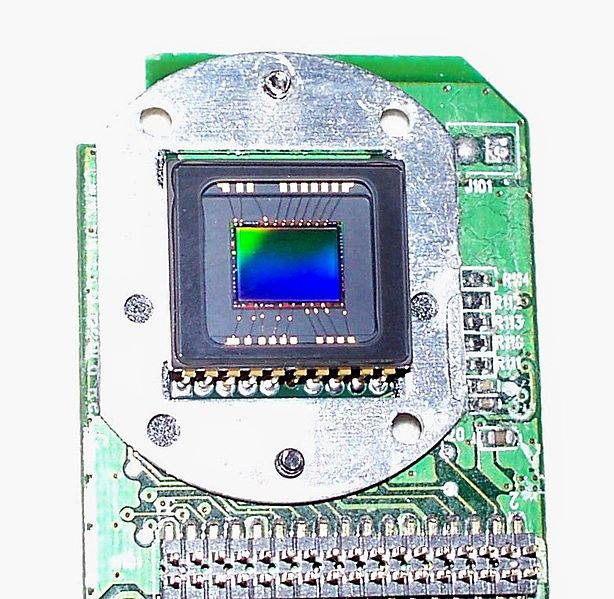
\includegraphics[width=0.4\textwidth]{images/ccd_chip.jpg}
  \caption{CCD from a 2.1 megapixel Hewlett-Packard digital camera (Wikipedia).}
  \label{fig:ccd_chip}
  \end{figure}

  \framebreak

   \begin{figure}[h!]
  \centering
  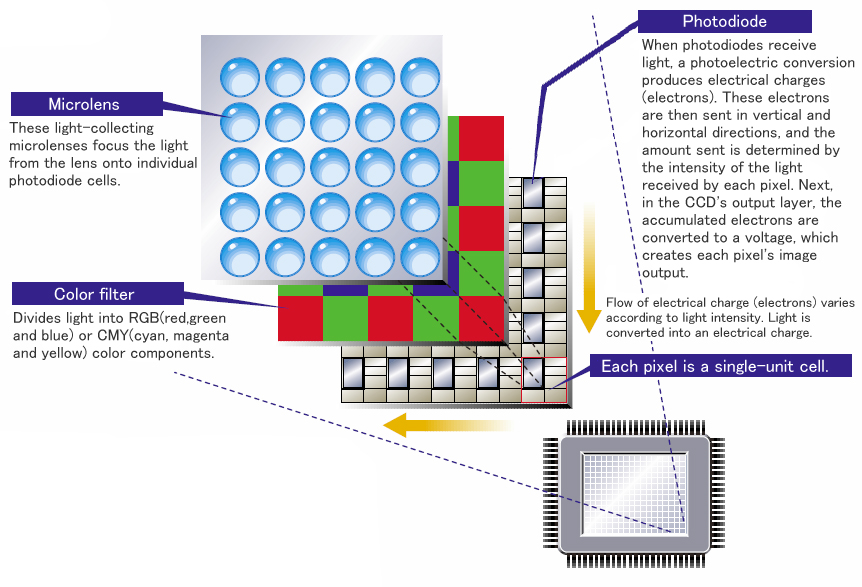
\includegraphics[width=0.6\textwidth]{images/ccd-panasonic.jpg}
  \caption{Funcionamento do CCD (\hrefcolor{https://av.jpn.support.panasonic.com/support/global/cs/dsc/knowhow/knowhow27.html}{Panasonic}).} 
  \label{fig:ccd-panasonic}
  \end{figure}

  \framebreak

  \begin{columns}[c]
  \column{.7\textwidth}
    \begin{figure}[h!]
    \centering
    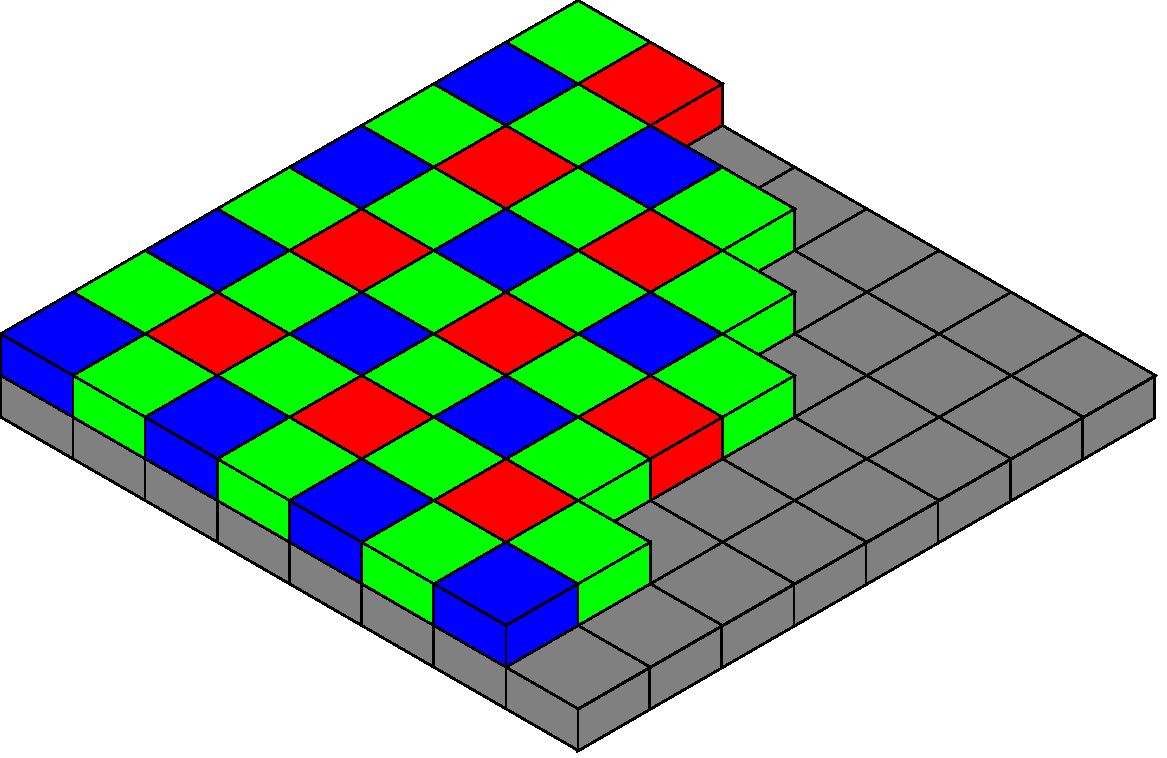
\includegraphics[width=0.5\textwidth]{images/bayer-patern.pdf}
    \caption{Máscara com Bayer sobre o CCD (Wikipedia).}
    \label{fig:bayer}
    \end{figure}
  \column{.3\textwidth}
    \begin{figure}[h!]
    \centering
    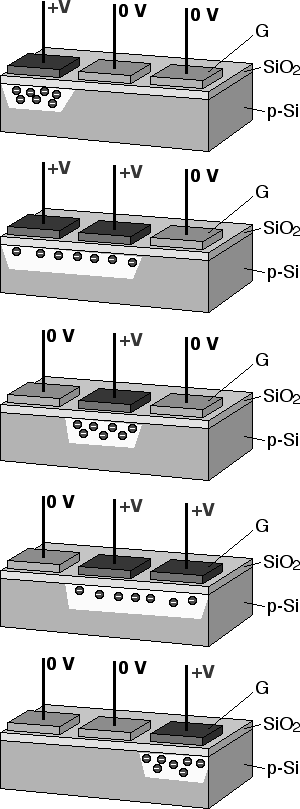
\includegraphics[width=0.5\textwidth]{images/ccd-charges.png}
    \caption{Deslocamento de cargas (Wikipedia).}
    \label{fig:charges}
    \end{figure}
  \end{columns}

  \framebreak

  \begin{figure}[h!]
  \centering
  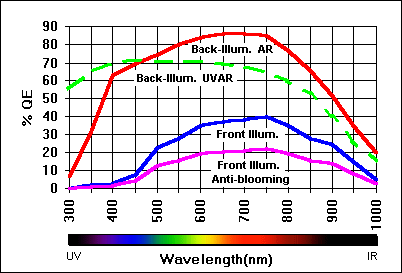
\includegraphics[width=0.5\textwidth]{images/quantum-eff.png}
  \caption{Eficiência quântica típica para CCDs \textit{front-} e \textit{back-illuminated} (\hrefcolor{http://www.astrosurf.com/re/ccdrev.html}{astrosurf}).}
  \label{fig:quantum}
  \end{figure}

  \framebreak

  \begin{columns}[c]
  \column{.65\textwidth}
    \begin{figure}[h!]
    \centering
    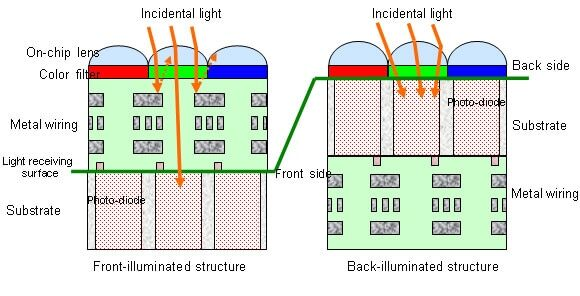
\includegraphics[width=0.9\textwidth]{images/front-back.jpg}
    \caption{Comparação entre estruturas \textit{front-illuminated} e \textit{back-illuminated} (\hrefcolor{https://www.sony.net/SonyInfo/News/Press/200806/08-069E/}{Sony}).}
    \label{fig:front-back}
    \end{figure}
  \column{.35\textwidth}
    \begin{figure}[h!]
    \centering
    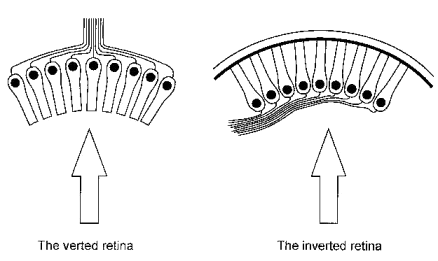
\includegraphics[width=\textwidth]{images/invretina.png}
    \caption{Comparação entre dois arranjos de fotorreceptores na retina (\hrefcolor{http://www.neuroanatomy.wisc.edu/selflearn/invertedretina.htm}{Gurney, P. W. V.}).}
    \label{fig:invretina}
    \end{figure} 
  \end{columns}

  \framebreak

  \bibentry{litwiller}

  
\includegraphics[width=0.3\textwidth]{images/qrcode-ccdcmos.pdf}
  \url{https://www2.cs.duke.edu/courses/fall11/cps274/papers/Littwiller01.pdf}

\end{frame}
\note{
Eficiência quântica de um dispositivo fotossensível é definida como o percentual de fótons incidentes
que irão produzir um par elétron-buraco.
\vspace{2ex}
Como a energia do fóton depende do seu comprimento de onda, a eficiência quântica é medida em diferentes
faixas de comprimento para assim caracterizar o dispositivo.
}

\begin{frame}[allowframebreaks]
  \frametitle{Ruído na aquisição de imagem}
  Fontes de ruído na aquisição da imagem:
  \begin{itemize}
  \item limitação na estatística de contagem dos fótons incidentes
  \item perdas durante o processo de deslocamento das cargas no chip CCD
  \item ruído eletrônico nos amplificadores e cabeamentos (ligações metálicas)
  \item interferências de fontes externas
  \end{itemize}

  \framebreak

  \begin{columns}[c]
  \column{.33\textwidth} 
    \begin{figure}[h!]
    \centering
    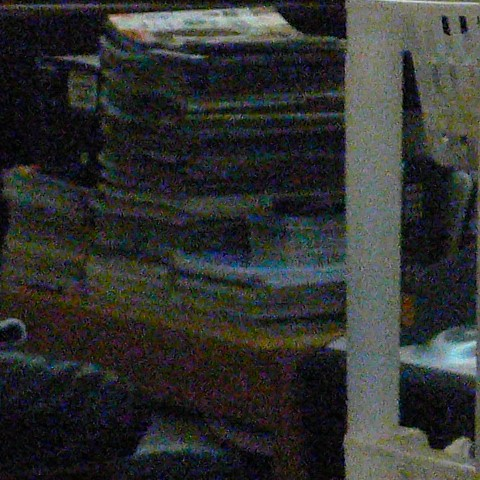
\includegraphics[width=0.9\textwidth]{images/highimgnoise.jpg}
    \caption{Ruído (Wikipedia).}
    \label{fig:highimgnoise}
    \end{figure}
  \column{.33\textwidth}
    \begin{figure}[h!]
    \centering
    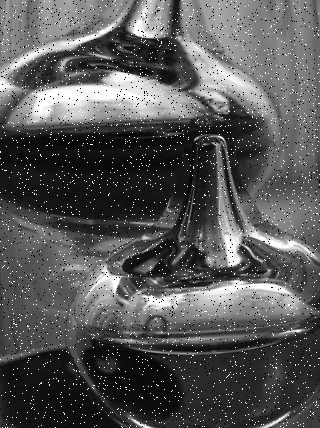
\includegraphics[width=0.8\textwidth]{images/saltandpepper.png}
    \caption{Ruído sal e pimenta (\textit{salt and pepper}) (Wikipedia).}
    \label{fig:saltandpepper}
    \end{figure}
  \column{.33\textwidth}
    \begin{figure}[h!]
    \centering
    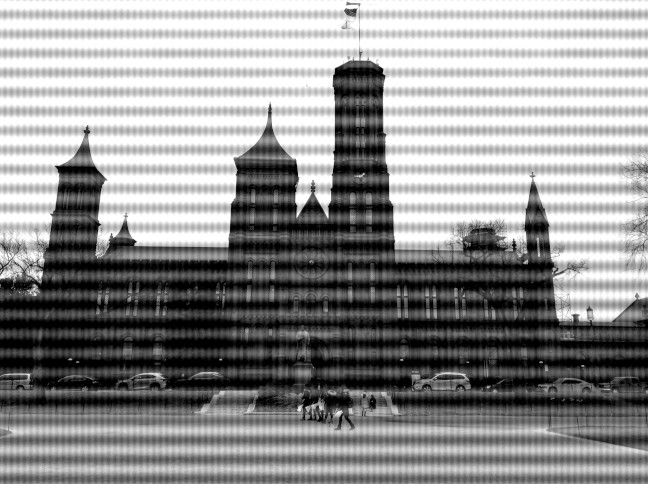
\includegraphics[width=\textwidth]{images/smithsonian-castle.jpg}
    \caption{Ruído periódico (Wikipedia).}
    \label{fig:smithsonian-castle}
    \end{figure}
  \end{columns}


  \framebreak

  \begin{columns}[c]
  \column{.33\textwidth}
    \begin{figure}[h!]
    \centering
    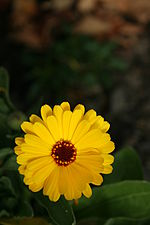
\includegraphics[width=0.6\textwidth]{images/comparison01.jpg}
    \caption{ISO 100, f/5.6, 1/350 s (Wikipedia).}
    \label{fig:comparison01}
    \end{figure}
 
  \column{.33\textwidth}
    \begin{figure}[h!]
    \centering
    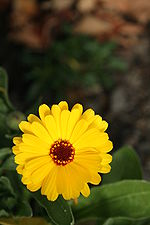
\includegraphics[width=0.6\textwidth]{images/comparison02.jpg}
    \caption{ISO 1600, f/5.6, 1/4000 s (Wikipedia).}
    \label{fig:comparison02}
    \end{figure}
 
  \column{.33\textwidth}
    \begin{figure}[h!]
    \centering
    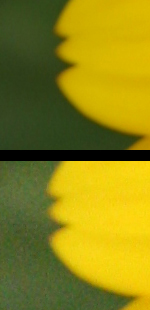
\includegraphics[width=0.5\textwidth]{images/comparison03.jpg}
    \caption{Comparação (Wikipedia).}
    \label{fig:comparison03}
    \end{figure}
 
  \end{columns}

  \framebreak

  Diferentes abordagens podem ser utilizadas para reduzir ruídos da imagem:
  \begin{itemize}
  \item sensores com maior área
  \item sensores com maior eficiência quântica
  \item menor temperatura
  \item projeto da câmera e sensor
  \item \textit{pixel binning}
  \item empilhamento de fotos (\textit{stacking})
  \item subtração do quadro de obscuridade (\textit{dark-frame subtraction})
  \item filtros digitais
  \end{itemize}
\end{frame}
\note{

\url{https://en.wikipedia.org/wiki/Dark-frame_subtraction}

\url{https://en.wikipedia.org/wiki/Focus_stacking}

}
\note{
``Signal-to-noise ratio (S/N) is one of the most important parameters to be considered when specifying a CCD camera for scientific applications. Three sources contribute to this ratio: photon, dark, and readout noise. Although many of these noise sources can be reduced by camera design and cooling methods, photon noise or photon shot noise—the inherent natural variation of incident photon flux—cannot be reduced by camera design. 

\url{https://www.vision-systems.com/cameras-accessories/image-sensors/article/16739105/scientificgrade-imagers-boost-ccd-sensitivity}
}
\note{
``Unlike photon noise, dark noise within a CCD is produced by electrons thermally generated within the structure of the CCD. Because the largest contribution to this dark current results from the interface between the silicon dioxide (SiO2) and the epitaxial silicon (Si) layer within the CCD, full-frame CCDs can be operated in multiphase pinned mode (MPP) to reduce this effect. The Si/SiO2 interface at the surface of the CCD is pinned at the substrate potential, directing signal charge away from the Si/SiO2 interface toward the buried n-channel. This reduces dark noise, increases charge-transfer efficiency, and increases pixel-to-pixel uniformity. ''

\url{https://www.vision-systems.com/cameras-accessories/image-sensors/article/16739105/scientificgrade-imagers-boost-ccd-sensitivity}
}
\note{
``Due to impurities in a CCD's silicon layer, some pixels suffer from dark current more than others. These so-called "hot pixels" build up thermal electrons at a much faster rate than the majority of pixels in the CCD. To reduce dark current caused by these pixels and others across the device, the CCD can be cooled. To accomplish this, the sensors used in scientific-quality cameras are cooled either by forced-air, thermoelectric (using Peltier coolers), or cryogenic means. For every 6°C reduction of temperature, dark current reduces by a factor of two. ''

\url{https://www.vision-systems.com/cameras-accessories/image-sensors/article/16739105/scientificgrade-imagers-boost-ccd-sensitivity}
}

\begin{frame}[allowframebreaks]
  \frametitle{Profundidade de Cor}
  Profundidade de cor (\emph{color depth} ou \emph{bit depth})
  é o número de bits utilizado para representar a cor em um único pixel em uma imagem bitmap.
  Espesso em bit por pixel (bpp). Este valor é limitado pelo quantizador na aquisição da imagem.

  \vspace{0.5cm}
  A profundidade de cor é apenas um aspecto da representação de cor, expressando o quão fina é
  a representação de uma cor (número de níveis). Outro aspecto importante é a extensão (gamut).

  \framebreak

  \begin{columns}[T]
  \column{.2\textwidth}
    \begin{figure}[h!]
    \centering
    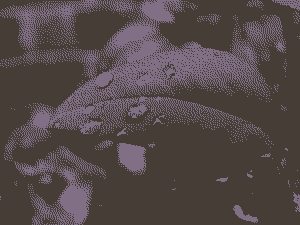
\includegraphics[width=\textwidth]{images/colordepth-1bit.png}
    \caption{1 bit (2 cores) (Wikipedia).}
    \label{fig:colordepth-1bit}
    \end{figure}
  \column{.2\textwidth}
    \begin{figure}[h!]
    \centering
    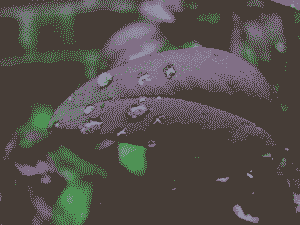
\includegraphics[width=\textwidth]{images/colordepth-2bit.png}
    \caption{2 bit (4 cores) (Wikipedia).}
    \label{fig:colordepth-2bit}
    \end{figure}
  \column{.2\textwidth}
    \begin{figure}[h!]
    \centering
    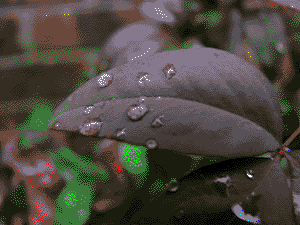
\includegraphics[width=\textwidth]{images/colordepth-4bit.png}
    \caption{4 bit (16 cores) (Wikipedia).}
    \label{fig:colordepth-4bit}
    \end{figure}
  \column{.2\textwidth}
    \begin{figure}[h!]
    \centering
    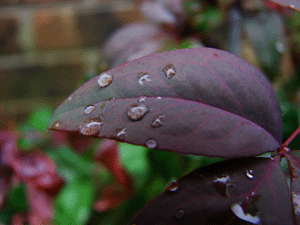
\includegraphics[width=\textwidth]{images/colordepth-8bit.png}
    \caption{8 bit (256 cores) (Wikipedia).}
    \label{fig:colordepth-8bit}
    \end{figure} 
  \column{.2\textwidth}
    \begin{figure}[h!]
    \centering
    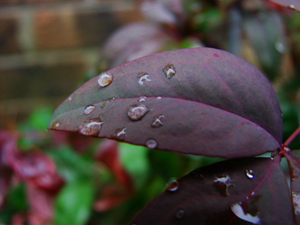
\includegraphics[width=\textwidth]{images/colordepth-24bit.png}
    \caption{24 bit (16.777.216 cores) (Wikipedia).}
    \label{fig:colordepth-24bit}
    \end{figure}  
  \end{columns}
\end{frame}
